\documentclass[1p]{elsarticle_modified}
%\bibliographystyle{elsarticle-num}

%\usepackage[colorlinks]{hyperref}
%\usepackage{abbrmath_seonhwa} %\Abb, \Ascr, \Acal ,\Abf, \Afrak
\usepackage{amsfonts}
\usepackage{amssymb}
\usepackage{amsmath}
\usepackage{amsthm}
\usepackage{scalefnt}
\usepackage{amsbsy}
\usepackage{kotex}
\usepackage{caption}
\usepackage{subfig}
\usepackage{color}
\usepackage{graphicx}
\usepackage{xcolor} %% white, black, red, green, blue, cyan, magenta, yellow
\usepackage{float}
\usepackage{setspace}
\usepackage{hyperref}

\usepackage{tikz}
\usetikzlibrary{arrows}

\usepackage{multirow}
\usepackage{array} % fixed length table
\usepackage{hhline}

%%%%%%%%%%%%%%%%%%%%%
\makeatletter
\renewcommand*\env@matrix[1][\arraystretch]{%
	\edef\arraystretch{#1}%
	\hskip -\arraycolsep
	\let\@ifnextchar\new@ifnextchar
	\array{*\c@MaxMatrixCols c}}
\makeatother %https://tex.stackexchange.com/questions/14071/how-can-i-increase-the-line-spacing-in-a-matrix
%%%%%%%%%%%%%%%

\usepackage[normalem]{ulem}

\newcommand{\msout}[1]{\ifmmode\text{\sout{\ensuremath{#1}}}\else\sout{#1}\fi}
%SOURCE: \msout is \stkout macro in https://tex.stackexchange.com/questions/20609/strikeout-in-math-mode

\newcommand{\cancel}[1]{
	\ifmmode
	{\color{red}\msout{#1}}
	\else
	{\color{red}\sout{#1}}
	\fi
}

\newcommand{\add}[1]{
	{\color{blue}\uwave{#1}}
}

\newcommand{\replace}[2]{
	\ifmmode
	{\color{red}\msout{#1}}{\color{blue}\uwave{#2}}
	\else
	{\color{red}\sout{#1}}{\color{blue}\uwave{#2}}
	\fi
}

\newcommand{\Sol}{\mathcal{S}} %segment
\newcommand{\D}{D} %diagram
\newcommand{\A}{\mathcal{A}} %arc


%%%%%%%%%%%%%%%%%%%%%%%%%%%%%5 test

\def\sl{\operatorname{\textup{SL}}(2,\Cbb)}
\def\psl{\operatorname{\textup{PSL}}(2,\Cbb)}
\def\quan{\mkern 1mu \triangleright \mkern 1mu}

\theoremstyle{definition}
\newtheorem{thm}{Theorem}[section]
\newtheorem{prop}[thm]{Proposition}
\newtheorem{lem}[thm]{Lemma}
\newtheorem{ques}[thm]{Question}
\newtheorem{cor}[thm]{Corollary}
\newtheorem{defn}[thm]{Definition}
\newtheorem{exam}[thm]{Example}
\newtheorem{rmk}[thm]{Remark}
\newtheorem{alg}[thm]{Algorithm}

\newcommand{\I}{\sqrt{-1}}
\begin{document}

%\begin{frontmatter}
%
%\title{Boundary parabolic representations of knots up to 8 crossings}
%
%%% Group authors per affiliation:
%\author{Yunhi Cho} 
%\address{Department of Mathematics, University of Seoul, Seoul, Korea}
%\ead{yhcho@uos.ac.kr}
%
%
%\author{Seonhwa Kim} %\fnref{s_kim}}
%\address{Center for Geometry and Physics, Institute for Basic Science, Pohang, 37673, Korea}
%\ead{ryeona17@ibs.re.kr}
%
%\author{Hyuk Kim}
%\address{Department of Mathematical Sciences, Seoul National University, Seoul 08826, Korea}
%\ead{hyukkim@snu.ac.kr}
%
%\author{Seokbeom Yoon}
%\address{Department of Mathematical Sciences, Seoul National University, Seoul, 08826,  Korea}
%\ead{sbyoon15@snu.ac.kr}
%
%\begin{abstract}
%We find all boundary parabolic representation of knots up to 8 crossings.
%
%\end{abstract}
%\begin{keyword}
%    \MSC[2010] 57M25 
%\end{keyword}
%
%\end{frontmatter}

%\linenumbers
%\tableofcontents
%
\newcommand\colored[1]{\textcolor{white}{\rule[-0.35ex]{0.8em}{1.4ex}}\kern-0.8em\color{red} #1}%
%\newcommand\colored[1]{\textcolor{white}{ #1}\kern-2.17ex	\textcolor{white}{ #1}\kern-1.81ex	\textcolor{white}{ #1}\kern-2.15ex\color{red}#1	}

{\Large $\underline{12a_{0854}~(K12a_{0854})}$}

\setlength{\tabcolsep}{10pt}
\renewcommand{\arraystretch}{1.6}
\vspace{1cm}\begin{tabular}{m{100pt}>{\centering\arraybackslash}m{274pt}}
\multirow{5}{120pt}{
	\centering
	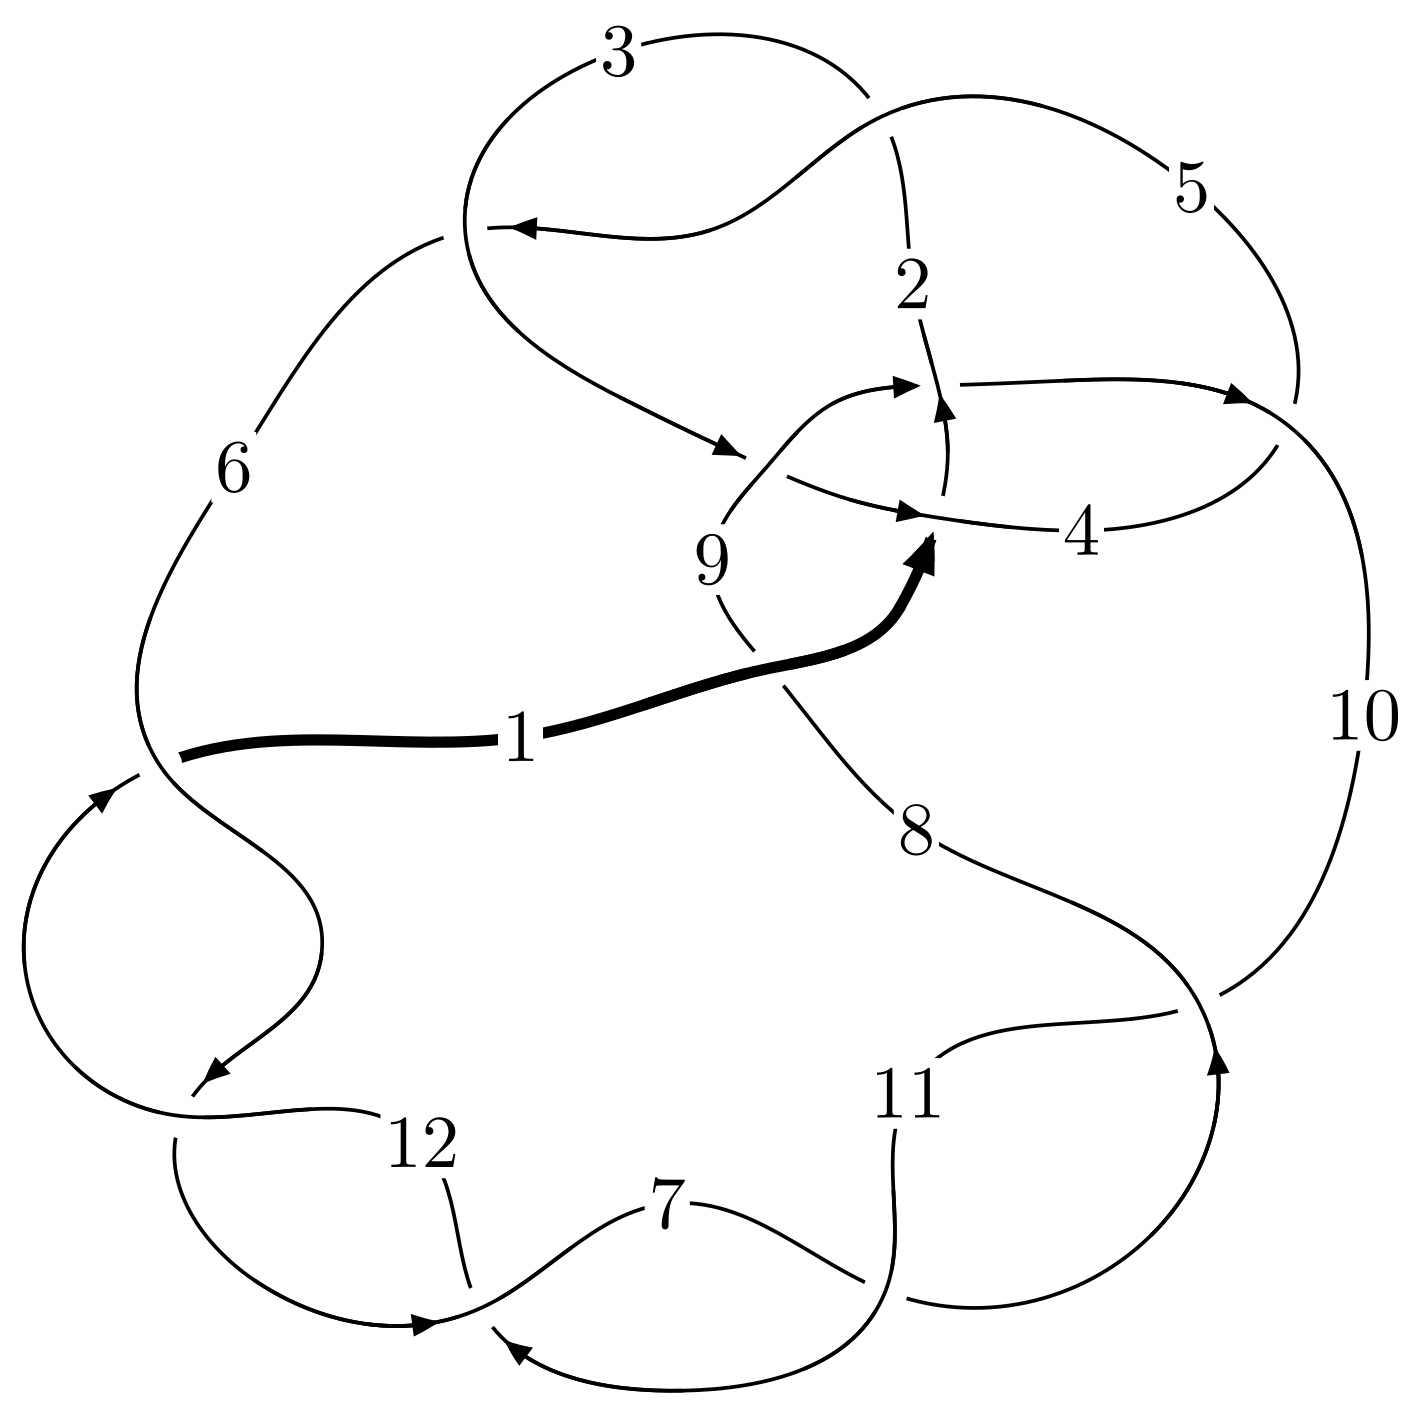
\includegraphics[width=112pt]{../../../GIT/diagram.site/Diagrams/png/1655_12a_0854.png}\\
\ \ \ A knot diagram\footnotemark}&
\allowdisplaybreaks
\textbf{Linearized knot diagam} \\
\cline{2-2}
 &
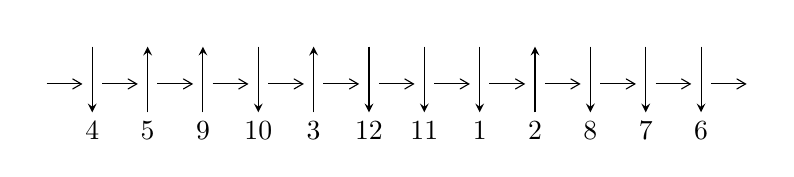
\begin{tikzpicture}[x=20pt, y=17pt]
	% nodes
	\node (C0) at (0, 0) {};
	\node (C1) at (1, 0) {};
	\node (C1U) at (1, +1) {};
	\node (C1D) at (1, -1) {4};

	\node (C2) at (2, 0) {};
	\node (C2U) at (2, +1) {};
	\node (C2D) at (2, -1) {5};

	\node (C3) at (3, 0) {};
	\node (C3U) at (3, +1) {};
	\node (C3D) at (3, -1) {9};

	\node (C4) at (4, 0) {};
	\node (C4U) at (4, +1) {};
	\node (C4D) at (4, -1) {10};

	\node (C5) at (5, 0) {};
	\node (C5U) at (5, +1) {};
	\node (C5D) at (5, -1) {3};

	\node (C6) at (6, 0) {};
	\node (C6U) at (6, +1) {};
	\node (C6D) at (6, -1) {12};

	\node (C7) at (7, 0) {};
	\node (C7U) at (7, +1) {};
	\node (C7D) at (7, -1) {11};

	\node (C8) at (8, 0) {};
	\node (C8U) at (8, +1) {};
	\node (C8D) at (8, -1) {1};

	\node (C9) at (9, 0) {};
	\node (C9U) at (9, +1) {};
	\node (C9D) at (9, -1) {2};

	\node (C10) at (10, 0) {};
	\node (C10U) at (10, +1) {};
	\node (C10D) at (10, -1) {8};

	\node (C11) at (11, 0) {};
	\node (C11U) at (11, +1) {};
	\node (C11D) at (11, -1) {7};

	\node (C12) at (12, 0) {};
	\node (C12U) at (12, +1) {};
	\node (C12D) at (12, -1) {6};
	\node (C13) at (13, 0) {};

	% arrows
	\draw[->,>={angle 60}]
	(C0) edge (C1) (C1) edge (C2) (C2) edge (C3) (C3) edge (C4) (C4) edge (C5) (C5) edge (C6) (C6) edge (C7) (C7) edge (C8) (C8) edge (C9) (C9) edge (C10) (C10) edge (C11) (C11) edge (C12) (C12) edge (C13) ;	\draw[->,>=stealth]
	(C1U) edge (C1D) (C2D) edge (C2U) (C3D) edge (C3U) (C4U) edge (C4D) (C5D) edge (C5U) (C6U) edge (C6D) (C7U) edge (C7D) (C8U) edge (C8D) (C9D) edge (C9U) (C10U) edge (C10D) (C11U) edge (C11D) (C12U) edge (C12D) ;
	\end{tikzpicture} \\
\hhline{~~} \\& 
\textbf{Solving Sequence} \\ \cline{2-2} 
 &
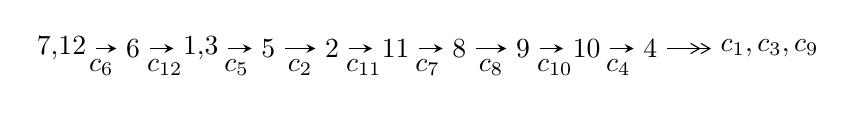
\begin{tikzpicture}[x=23pt, y=7pt]
	% node
	\node (A0) at (-1/8, 0) {7,12};
	\node (A1) at (1, 0) {6};
	\node (A2) at (33/16, 0) {1,3};
	\node (A3) at (25/8, 0) {5};
	\node (A4) at (33/8, 0) {2};
	\node (A5) at (41/8, 0) {11};
	\node (A6) at (49/8, 0) {8};
	\node (A7) at (57/8, 0) {9};
	\node (A8) at (65/8, 0) {10};
	\node (A9) at (73/8, 0) {4};
	\node (C1) at (1/2, -1) {$c_{6}$};
	\node (C2) at (3/2, -1) {$c_{12}$};
	\node (C3) at (21/8, -1) {$c_{5}$};
	\node (C4) at (29/8, -1) {$c_{2}$};
	\node (C5) at (37/8, -1) {$c_{11}$};
	\node (C6) at (45/8, -1) {$c_{7}$};
	\node (C7) at (53/8, -1) {$c_{8}$};
	\node (C8) at (61/8, -1) {$c_{10}$};
	\node (C9) at (69/8, -1) {$c_{4}$};
	\node (A10) at (11, 0) {$c_{1},c_{3},c_{9}$};

	% edge
	\draw[->,>=stealth]	
	(A0) edge (A1) (A1) edge (A2) (A2) edge (A3) (A3) edge (A4) (A4) edge (A5) (A5) edge (A6) (A6) edge (A7) (A7) edge (A8) (A8) edge (A9) ;
	\draw[->>,>={angle 60}]	
	(A9) edge (A10);
\end{tikzpicture} \\ 

\end{tabular} \\

\footnotetext{
The image of knot diagram is generated by the software ``\textbf{Draw programme}" developed by Andrew Bartholomew(\url{http://www.layer8.co.uk/maths/draw/index.htm\#Running-draw}), where we modified some parts for our purpose(\url{https://github.com/CATsTAILs/LinksPainter}).
}\phantom \\ \newline 
\centering \textbf{Ideals for irreducible components\footnotemark of $X_{\text{par}}$} 
 
\begin{align*}
I^u_{1}&=\langle 
-4.18772\times10^{18} u^{65}+6.44102\times10^{20} u^{64}+\cdots+7.93709\times10^{20} b-6.29281\times10^{16},\\
\phantom{I^u_{1}}&\phantom{= \langle  }-2.93073\times10^{19} u^{65}+4.50916\times10^{21} u^{64}+\cdots+5.55596\times10^{21} a-5.64900\times10^{21},\;u^{66}+u^{65}+\cdots+3 u+1\rangle \\
\\
\end{align*}
\raggedright * 1 irreducible components of $\dim_{\mathbb{C}}=0$, with total 66 representations.\\
\footnotetext{All coefficients of polynomials are rational numbers. But the coefficients are sometimes approximated in decimal forms when there is not enough margin.}
\newpage
\renewcommand{\arraystretch}{1}
\centering \section*{I. $I^u_{1}= \langle -4.19\times10^{18} u^{65}+6.44\times10^{20} u^{64}+\cdots+7.94\times10^{20} b-6.29\times10^{16},\;-2.93\times10^{19} u^{65}+4.51\times10^{21} u^{64}+\cdots+5.56\times10^{21} a-5.65\times10^{21},\;u^{66}+u^{65}+\cdots+3 u+1 \rangle$}
\flushleft \textbf{(i) Arc colorings}\\
\begin{tabular}{m{7pt} m{180pt} m{7pt} m{180pt} }
\flushright $a_{7}=$&$\begin{pmatrix}1\\0\end{pmatrix}$ \\
\flushright $a_{12}=$&$\begin{pmatrix}0\\u\end{pmatrix}$ \\
\flushright $a_{6}=$&$\begin{pmatrix}1\\- u^2\end{pmatrix}$ \\
\flushright $a_{1}=$&$\begin{pmatrix}- u\\u^3+u\end{pmatrix}$ \\
\flushright $a_{3}=$&$\begin{pmatrix}0.00527494 u^{65}-0.811590 u^{64}+\cdots+3.23371 u+1.01675\\0.00527615 u^{65}-0.811510 u^{64}+\cdots-3.18309 u+0.0000792836\end{pmatrix}$ \\
\flushright $a_{5}=$&$\begin{pmatrix}-0.00442903 u^{65}-0.736691 u^{64}+\cdots+2.32738 u+1.74996\\-0.00442982 u^{65}-0.736731 u^{64}+\cdots-3.25012 u-0.0000393662\end{pmatrix}$ \\
\flushright $a_{2}=$&$\begin{pmatrix}-0.00273721 u^{65}-0.833252 u^{64}+\cdots+1.44957 u-0.716626\\-0.00273716 u^{65}-0.833212 u^{64}+\cdots-0.116545 u+0.0000404686\end{pmatrix}$ \\
\flushright $a_{11}=$&$\begin{pmatrix}u\\u\end{pmatrix}$ \\
\flushright $a_{8}=$&$\begin{pmatrix}u^2+1\\u^2\end{pmatrix}$ \\
\flushright $a_{9}=$&$\begin{pmatrix}- u^6-3 u^4+1\\u^8+4 u^6+4 u^4+2 u^2\end{pmatrix}$ \\
\flushright $a_{10}=$&$\begin{pmatrix}u^3+2 u\\u^3+u\end{pmatrix}$ \\
\flushright $a_{4}=$&$\begin{pmatrix}-0.000766897 u^{65}-0.0917424 u^{64}+\cdots+2.32749 u+1.75000\\-0.000767003 u^{65}-0.0917456 u^{64}+\cdots-3.25001 u-3.08525\times10^{-6}\end{pmatrix}$\\&\end{tabular}
\flushleft \textbf{(ii) Obstruction class $= -1$}\\~\\
\flushleft \textbf{(iii) Cusp Shapes $= -\frac{17667926048719462539416}{5555960082374174168269} u^{65}-\frac{1888758008650562826900}{793708583196310595467} u^{64}+\cdots+\frac{30639294781679213832508}{5555960082374174168269} u+\frac{25448149131766158381870}{5555960082374174168269}$}\\~\\
\newpage\renewcommand{\arraystretch}{1}
\flushleft \textbf{(iv) u-Polynomials at the component}\newline \\
\begin{tabular}{m{50pt}|m{274pt}}
Crossings & \hspace{64pt}u-Polynomials at each crossing \\
\hline $$\begin{aligned}c_{1}\end{aligned}$$&$\begin{aligned}
&u^{66}-11 u^{65}+\cdots- u+1
\end{aligned}$\\
\hline $$\begin{aligned}c_{2},c_{5}\end{aligned}$$&$\begin{aligned}
&u^{66}+u^{65}+\cdots+11 u+1
\end{aligned}$\\
\hline $$\begin{aligned}c_{3}\end{aligned}$$&$\begin{aligned}
&u^{66}- u^{65}+\cdots+116 u-8
\end{aligned}$\\
\hline $$\begin{aligned}c_{4}\end{aligned}$$&$\begin{aligned}
&u^{66}+u^{65}+\cdots-39 u+19
\end{aligned}$\\
\hline $$\begin{aligned}c_{6},c_{7},c_{10}\\c_{11},c_{12}\end{aligned}$$&$\begin{aligned}
&u^{66}- u^{65}+\cdots-3 u+1
\end{aligned}$\\
\hline $$\begin{aligned}c_{8}\end{aligned}$$&$\begin{aligned}
&u^{66}- u^{65}+\cdots-1149 u+1069
\end{aligned}$\\
\hline $$\begin{aligned}c_{9}\end{aligned}$$&$\begin{aligned}
&u^{66}+3 u^{65}+\cdots+u+1
\end{aligned}$\\
\hline
\end{tabular}\\~\\
\newpage\renewcommand{\arraystretch}{1}
\flushleft \textbf{(v) Riley Polynomials at the component}\newline \\
\begin{tabular}{m{50pt}|m{274pt}}
Crossings & \hspace{64pt}Riley Polynomials at each crossing \\
\hline $$\begin{aligned}c_{1}\end{aligned}$$&$\begin{aligned}
&y^{66}-3 y^{65}+\cdots-11 y+1
\end{aligned}$\\
\hline $$\begin{aligned}c_{2},c_{5}\end{aligned}$$&$\begin{aligned}
&y^{66}-43 y^{65}+\cdots-11 y+1
\end{aligned}$\\
\hline $$\begin{aligned}c_{3}\end{aligned}$$&$\begin{aligned}
&y^{66}+53 y^{65}+\cdots-18384 y+64
\end{aligned}$\\
\hline $$\begin{aligned}c_{4}\end{aligned}$$&$\begin{aligned}
&y^{66}+69 y^{65}+\cdots+17213 y+361
\end{aligned}$\\
\hline $$\begin{aligned}c_{6},c_{7},c_{10}\\c_{11},c_{12}\end{aligned}$$&$\begin{aligned}
&y^{66}+85 y^{65}+\cdots-3 y+1
\end{aligned}$\\
\hline $$\begin{aligned}c_{8}\end{aligned}$$&$\begin{aligned}
&y^{66}-3 y^{65}+\cdots+10590597 y+1142761
\end{aligned}$\\
\hline $$\begin{aligned}c_{9}\end{aligned}$$&$\begin{aligned}
&y^{66}-11 y^{65}+\cdots-3 y+1
\end{aligned}$\\
\hline
\end{tabular}\\~\\
\newpage\flushleft \textbf{(vi) Complex Volumes and Cusp Shapes}
$$\begin{array}{c|c|c}  
\text{Solutions to }I^u_{1}& \I (\text{vol} + \sqrt{-1}CS) & \text{Cusp shape}\\
 \hline 
\begin{aligned}
u &= -0.320550 + 0.945885 I \\
a &= -1.063260 - 0.335944 I \\
b &= -0.685686 + 0.247428 I\end{aligned}
 & \phantom{-}0.80470 + 7.26585 I & \phantom{-0.000000 } 0 \\ \hline\begin{aligned}
u &= -0.320550 - 0.945885 I \\
a &= -1.063260 + 0.335944 I \\
b &= -0.685686 - 0.247428 I\end{aligned}
 & \phantom{-}0.80470 - 7.26585 I & \phantom{-0.000000 } 0 \\ \hline\begin{aligned}
u &= -0.259011 + 0.962168 I \\
a &= -2.13062 + 1.40357 I \\
b &= -1.20371 + 0.85170 I\end{aligned}
 & \phantom{-}5.56803 + 4.96269 I & \phantom{-0.000000 } 0 \\ \hline\begin{aligned}
u &= -0.259011 - 0.962168 I \\
a &= -2.13062 - 1.40357 I \\
b &= -1.20371 - 0.85170 I\end{aligned}
 & \phantom{-}5.56803 - 4.96269 I & \phantom{-0.000000 } 0 \\ \hline\begin{aligned}
u &= -0.191816 + 0.964958 I \\
a &= -1.81489 + 1.32945 I \\
b &= -0.589613 + 0.207069 I\end{aligned}
 & \phantom{-}6.29804 + 1.24184 I & \phantom{-0.000000 } 0 \\ \hline\begin{aligned}
u &= -0.191816 - 0.964958 I \\
a &= -1.81489 - 1.32945 I \\
b &= -0.589613 - 0.207069 I\end{aligned}
 & \phantom{-}6.29804 - 1.24184 I & \phantom{-0.000000 } 0 \\ \hline\begin{aligned}
u &= \phantom{-}0.238535 + 0.917340 I \\
a &= -3.28193 - 3.26906 I \\
b &= -2.96619 - 1.22505 I\end{aligned}
 & \phantom{-}3.70547 - 2.54918 I & \phantom{-0.000000 } 0 \\ \hline\begin{aligned}
u &= \phantom{-}0.238535 - 0.917340 I \\
a &= -3.28193 + 3.26906 I \\
b &= -2.96619 + 1.22505 I\end{aligned}
 & \phantom{-}3.70547 + 2.54918 I & \phantom{-0.000000 } 0 \\ \hline\begin{aligned}
u &= -0.365061 + 0.991459 I \\
a &= \phantom{-}2.00582 - 1.50902 I \\
b &= \phantom{-}1.44867 - 0.39349 I\end{aligned}
 & \phantom{-}4.89146 + 13.26630 I & \phantom{-0.000000 } 0 \\ \hline\begin{aligned}
u &= -0.365061 - 0.991459 I \\
a &= \phantom{-}2.00582 + 1.50902 I \\
b &= \phantom{-}1.44867 + 0.39349 I\end{aligned}
 & \phantom{-}4.89146 - 13.26630 I & \phantom{-0.000000 } 0\\
 \hline 
 \end{array}$$\newpage$$\begin{array}{c|c|c}  
\text{Solutions to }I^u_{1}& \I (\text{vol} + \sqrt{-1}CS) & \text{Cusp shape}\\
 \hline 
\begin{aligned}
u &= \phantom{-}0.303217 + 0.885615 I \\
a &= \phantom{-}0.315243 - 0.014355 I \\
b &= \phantom{-}0.100769 - 0.435003 I\end{aligned}
 & \phantom{-}1.36354 - 2.78002 I & \phantom{-0.000000 } 0 \\ \hline\begin{aligned}
u &= \phantom{-}0.303217 - 0.885615 I \\
a &= \phantom{-}0.315243 + 0.014355 I \\
b &= \phantom{-}0.100769 + 0.435003 I\end{aligned}
 & \phantom{-}1.36354 + 2.78002 I & \phantom{-0.000000 } 0 \\ \hline\begin{aligned}
u &= -0.063187 + 0.925648 I \\
a &= \phantom{-}0.363461 + 0.619325 I \\
b &= \phantom{-}0.744300 - 0.157815 I\end{aligned}
 & \phantom{-}3.48184 - 1.42801 I & \phantom{-0.000000 } 0 \\ \hline\begin{aligned}
u &= -0.063187 - 0.925648 I \\
a &= \phantom{-}0.363461 - 0.619325 I \\
b &= \phantom{-}0.744300 + 0.157815 I\end{aligned}
 & \phantom{-}3.48184 + 1.42801 I & \phantom{-0.000000 } 0 \\ \hline\begin{aligned}
u &= \phantom{-}0.363535 + 1.037990 I \\
a &= \phantom{-}1.60954 + 0.96579 I \\
b &= \phantom{-}1.224800 - 0.068819 I\end{aligned}
 & \phantom{-}3.57327 - 5.06511 I & \phantom{-0.000000 } 0 \\ \hline\begin{aligned}
u &= \phantom{-}0.363535 - 1.037990 I \\
a &= \phantom{-}1.60954 - 0.96579 I \\
b &= \phantom{-}1.224800 + 0.068819 I\end{aligned}
 & \phantom{-}3.57327 + 5.06511 I & \phantom{-0.000000 } 0 \\ \hline\begin{aligned}
u &= \phantom{-}0.167951 + 0.857359 I \\
a &= \phantom{-}0.465621 + 1.190710 I \\
b &= \phantom{-}1.40004 + 0.77822 I\end{aligned}
 & \phantom{-}2.98373 - 1.62353 I & \phantom{-}4.86404 + 6.61880 I \\ \hline\begin{aligned}
u &= \phantom{-}0.167951 - 0.857359 I \\
a &= \phantom{-}0.465621 - 1.190710 I \\
b &= \phantom{-}1.40004 - 0.77822 I\end{aligned}
 & \phantom{-}2.98373 + 1.62353 I & \phantom{-}4.86404 - 6.61880 I \\ \hline\begin{aligned}
u &= \phantom{-}0.457424 + 0.731064 I \\
a &= \phantom{-}0.725928 + 0.706575 I \\
b &= -0.201103 - 0.033272 I\end{aligned}
 & \phantom{-}1.12406 - 3.70601 I & \phantom{-0.000000 -}0. + 11.51127 I \\ \hline\begin{aligned}
u &= \phantom{-}0.457424 - 0.731064 I \\
a &= \phantom{-}0.725928 - 0.706575 I \\
b &= -0.201103 + 0.033272 I\end{aligned}
 & \phantom{-}1.12406 + 3.70601 I & \phantom{-0.000000 } 0. - 11.51127 I\\
 \hline 
 \end{array}$$\newpage$$\begin{array}{c|c|c}  
\text{Solutions to }I^u_{1}& \I (\text{vol} + \sqrt{-1}CS) & \text{Cusp shape}\\
 \hline 
\begin{aligned}
u &= -0.061425 + 1.191140 I \\
a &= \phantom{-}1.84871 - 0.38837 I \\
b &= \phantom{-}1.41998 + 0.05717 I\end{aligned}
 & \phantom{-}8.29302 - 4.76690 I & \phantom{-0.000000 } 0 \\ \hline\begin{aligned}
u &= -0.061425 - 1.191140 I \\
a &= \phantom{-}1.84871 + 0.38837 I \\
b &= \phantom{-}1.41998 - 0.05717 I\end{aligned}
 & \phantom{-}8.29302 + 4.76690 I & \phantom{-0.000000 } 0 \\ \hline\begin{aligned}
u &= -0.458535 + 0.561466 I \\
a &= \phantom{-}0.255118 - 0.554018 I \\
b &= -0.941274 + 0.566973 I\end{aligned}
 & \phantom{-}2.41285 - 6.45141 I & -0.54002 + 2.68736 I \\ \hline\begin{aligned}
u &= -0.458535 - 0.561466 I \\
a &= \phantom{-}0.255118 + 0.554018 I \\
b &= -0.941274 - 0.566973 I\end{aligned}
 & \phantom{-}2.41285 + 6.45141 I & -0.54002 - 2.68736 I \\ \hline\begin{aligned}
u &= -0.290297 + 0.626646 I \\
a &= \phantom{-}1.205330 - 0.394635 I \\
b &= \phantom{-}0.339995 - 0.557211 I\end{aligned}
 & -1.00030 - 1.44920 I & -4.20313 + 0.51290 I \\ \hline\begin{aligned}
u &= -0.290297 - 0.626646 I \\
a &= \phantom{-}1.205330 + 0.394635 I \\
b &= \phantom{-}0.339995 + 0.557211 I\end{aligned}
 & -1.00030 + 1.44920 I & -4.20313 - 0.51290 I \\ \hline\begin{aligned}
u &= \phantom{-}0.583780 + 0.292413 I \\
a &= \phantom{-}0.586657 + 0.798318 I \\
b &= -0.733275 - 0.248558 I\end{aligned}
 & -0.52146 - 1.81812 I & -11.1036 + 9.5392 I \\ \hline\begin{aligned}
u &= \phantom{-}0.583780 - 0.292413 I \\
a &= \phantom{-}0.586657 - 0.798318 I \\
b &= -0.733275 + 0.248558 I\end{aligned}
 & -0.52146 + 1.81812 I & -11.1036 - 9.5392 I \\ \hline\begin{aligned}
u &= \phantom{-}0.651823\phantom{ +0.000000I} \\
a &= -0.176116\phantom{ +0.000000I} \\
b &= -0.723296\phantom{ +0.000000I}\end{aligned}
 & -1.07816\phantom{ +0.000000I} & -15.1890\phantom{ +0.000000I} \\ \hline\begin{aligned}
u &= -0.600823 + 0.187862 I \\
a &= \phantom{-}0.18260 - 1.64994 I \\
b &= -0.988132 + 0.036198 I\end{aligned}
 & \phantom{-}1.26055 + 9.99441 I & -3.17960 - 8.12625 I\\
 \hline 
 \end{array}$$\newpage$$\begin{array}{c|c|c}  
\text{Solutions to }I^u_{1}& \I (\text{vol} + \sqrt{-1}CS) & \text{Cusp shape}\\
 \hline 
\begin{aligned}
u &= -0.600823 - 0.187862 I \\
a &= \phantom{-}0.18260 + 1.64994 I \\
b &= -0.988132 - 0.036198 I\end{aligned}
 & \phantom{-}1.26055 - 9.99441 I & -3.17960 + 8.12625 I \\ \hline\begin{aligned}
u &= -0.533895 + 0.131590 I \\
a &= -0.533306 + 1.262460 I \\
b &= -0.136821 + 0.638790 I\end{aligned}
 & -2.49763 + 4.35833 I & -7.38425 - 7.01489 I \\ \hline\begin{aligned}
u &= -0.533895 - 0.131590 I \\
a &= -0.533306 - 1.262460 I \\
b &= -0.136821 - 0.638790 I\end{aligned}
 & -2.49763 - 4.35833 I & -7.38425 + 7.01489 I \\ \hline\begin{aligned}
u &= \phantom{-}0.513633\phantom{ +0.000000I} \\
a &= \phantom{-}0.361156\phantom{ +0.000000I} \\
b &= -0.284384\phantom{ +0.000000I}\end{aligned}
 & -1.34771\phantom{ +0.000000I} & -8.70160\phantom{ +0.000000I} \\ \hline\begin{aligned}
u &= -0.431584 + 0.169963 I \\
a &= \phantom{-}0.27177 + 2.35884 I \\
b &= \phantom{-}0.813624 + 0.264792 I\end{aligned}
 & \phantom{-}2.09817 + 2.58100 I & -0.10269 - 8.35821 I \\ \hline\begin{aligned}
u &= -0.431584 - 0.169963 I \\
a &= \phantom{-}0.27177 - 2.35884 I \\
b &= \phantom{-}0.813624 - 0.264792 I\end{aligned}
 & \phantom{-}2.09817 - 2.58100 I & -0.10269 + 8.35821 I \\ \hline\begin{aligned}
u &= \phantom{-}0.258905 + 0.380359 I \\
a &= \phantom{-}0.834851 + 0.121731 I \\
b &= -0.074634 - 0.484044 I\end{aligned}
 & -0.402527 - 1.133020 I & -5.71641 + 5.32128 I \\ \hline\begin{aligned}
u &= \phantom{-}0.258905 - 0.380359 I \\
a &= \phantom{-}0.834851 - 0.121731 I \\
b &= -0.074634 + 0.484044 I\end{aligned}
 & -0.402527 + 1.133020 I & -5.71641 - 5.32128 I \\ \hline\begin{aligned}
u &= \phantom{-}0.410014 + 0.063112 I \\
a &= \phantom{-}0.31651 - 4.71230 I \\
b &= \phantom{-}0.659200 + 0.694375 I\end{aligned}
 & \phantom{-}0.701377 - 0.322381 I & \phantom{-}4.5634 - 19.7316 I \\ \hline\begin{aligned}
u &= \phantom{-}0.410014 - 0.063112 I \\
a &= \phantom{-}0.31651 + 4.71230 I \\
b &= \phantom{-}0.659200 - 0.694375 I\end{aligned}
 & \phantom{-}0.701377 + 0.322381 I & \phantom{-}4.5634 + 19.7316 I\\
 \hline 
 \end{array}$$\newpage$$\begin{array}{c|c|c}  
\text{Solutions to }I^u_{1}& \I (\text{vol} + \sqrt{-1}CS) & \text{Cusp shape}\\
 \hline 
\begin{aligned}
u &= \phantom{-}0.04843 + 1.59433 I \\
a &= \phantom{-}1.042930 + 0.100093 I \\
b &= \phantom{-}1.64649 + 0.53314 I\end{aligned}
 & \phantom{-}8.81067 - 5.43936 I & \phantom{-0.000000 } 0 \\ \hline\begin{aligned}
u &= \phantom{-}0.04843 - 1.59433 I \\
a &= \phantom{-}1.042930 - 0.100093 I \\
b &= \phantom{-}1.64649 - 0.53314 I\end{aligned}
 & \phantom{-}8.81067 + 5.43936 I & \phantom{-0.000000 } 0 \\ \hline\begin{aligned}
u &= -0.261393 + 0.254743 I \\
a &= \phantom{-}0.680829 + 1.108350 I \\
b &= \phantom{-}1.102630 - 0.201893 I\end{aligned}
 & \phantom{-}2.68024 - 0.40653 I & \phantom{-}3.06802 - 3.24326 I \\ \hline\begin{aligned}
u &= -0.261393 - 0.254743 I \\
a &= \phantom{-}0.680829 - 1.108350 I \\
b &= \phantom{-}1.102630 + 0.201893 I\end{aligned}
 & \phantom{-}2.68024 + 0.40653 I & \phantom{-}3.06802 + 3.24326 I \\ \hline\begin{aligned}
u &= -0.02226 + 1.64012 I \\
a &= \phantom{-}0.931045 + 0.007675 I \\
b &= \phantom{-}2.06715 - 0.75388 I\end{aligned}
 & \phantom{-}6.95676 - 0.72964 I & \phantom{-0.000000 } 0 \\ \hline\begin{aligned}
u &= -0.02226 - 1.64012 I \\
a &= \phantom{-}0.931045 - 0.007675 I \\
b &= \phantom{-}2.06715 + 0.75388 I\end{aligned}
 & \phantom{-}6.95676 + 0.72964 I & \phantom{-0.000000 } 0 \\ \hline\begin{aligned}
u &= \phantom{-}0.04369 + 1.69093 I \\
a &= -0.088591 + 0.936388 I \\
b &= \phantom{-}0.56172 + 2.91859 I\end{aligned}
 & \phantom{-}12.08540 - 2.44069 I & \phantom{-0.000000 } 0 \\ \hline\begin{aligned}
u &= \phantom{-}0.04369 - 1.69093 I \\
a &= -0.088591 - 0.936388 I \\
b &= \phantom{-}0.56172 - 2.91859 I\end{aligned}
 & \phantom{-}12.08540 + 2.44069 I & \phantom{-0.000000 } 0 \\ \hline\begin{aligned}
u &= \phantom{-}0.07604 + 1.68991 I \\
a &= \phantom{-}0.257142 + 0.020404 I \\
b &= \phantom{-}0.672101 - 0.399751 I\end{aligned}
 & \phantom{-}10.45740 - 4.23214 I & \phantom{-0.000000 } 0 \\ \hline\begin{aligned}
u &= \phantom{-}0.07604 - 1.68991 I \\
a &= \phantom{-}0.257142 - 0.020404 I \\
b &= \phantom{-}0.672101 + 0.399751 I\end{aligned}
 & \phantom{-}10.45740 + 4.23214 I & \phantom{-0.000000 } 0\\
 \hline 
 \end{array}$$\newpage$$\begin{array}{c|c|c}  
\text{Solutions to }I^u_{1}& \I (\text{vol} + \sqrt{-1}CS) & \text{Cusp shape}\\
 \hline 
\begin{aligned}
u &= \phantom{-}0.06014 + 1.69901 I \\
a &= -3.27791 - 2.08492 I \\
b &= -8.79298 - 5.45875 I\end{aligned}
 & \phantom{-}12.99110 - 3.71015 I & \phantom{-0.000000 } 0 \\ \hline\begin{aligned}
u &= \phantom{-}0.06014 - 1.69901 I \\
a &= -3.27791 + 2.08492 I \\
b &= -8.79298 + 5.45875 I\end{aligned}
 & \phantom{-}12.99110 + 3.71015 I & \phantom{-0.000000 } 0 \\ \hline\begin{aligned}
u &= -0.02854 + 1.70099 I \\
a &= -0.082212 + 0.726413 I \\
b &= \phantom{-}0.298235 + 1.131330 I\end{aligned}
 & \phantom{-}12.84170 - 0.97443 I & \phantom{-0.000000 } 0 \\ \hline\begin{aligned}
u &= -0.02854 - 1.70099 I \\
a &= -0.082212 - 0.726413 I \\
b &= \phantom{-}0.298235 - 1.131330 I\end{aligned}
 & \phantom{-}12.84170 + 0.97443 I & \phantom{-0.000000 } 0 \\ \hline\begin{aligned}
u &= -0.08226 + 1.70288 I \\
a &= -0.697707 - 0.726127 I \\
b &= -1.83993 - 1.06056 I\end{aligned}
 & \phantom{-}10.15510 + 8.84894 I & \phantom{-0.000000 } 0 \\ \hline\begin{aligned}
u &= -0.08226 - 1.70288 I \\
a &= -0.697707 + 0.726127 I \\
b &= -1.83993 + 1.06056 I\end{aligned}
 & \phantom{-}10.15510 - 8.84894 I & \phantom{-0.000000 } 0 \\ \hline\begin{aligned}
u &= -0.06632 + 1.70870 I \\
a &= -2.25962 + 0.63483 I \\
b &= -5.34135 + 2.11063 I\end{aligned}
 & \phantom{-}15.0454 + 6.2521 I & \phantom{-0.000000 } 0 \\ \hline\begin{aligned}
u &= -0.06632 - 1.70870 I \\
a &= -2.25962 - 0.63483 I \\
b &= -5.34135 - 2.11063 I\end{aligned}
 & \phantom{-}15.0454 - 6.2521 I & \phantom{-0.000000 } 0 \\ \hline\begin{aligned}
u &= -0.05073 + 1.70963 I \\
a &= -2.20674 + 0.93195 I \\
b &= -4.97480 + 1.99997 I\end{aligned}
 & \phantom{-}15.8171 + 2.2173 I & \phantom{-0.000000 } 0 \\ \hline\begin{aligned}
u &= -0.05073 - 1.70963 I \\
a &= -2.20674 - 0.93195 I \\
b &= -4.97480 - 1.99997 I\end{aligned}
 & \phantom{-}15.8171 - 2.2173 I & \phantom{-0.000000 } 0\\
 \hline 
 \end{array}$$\newpage$$\begin{array}{c|c|c}  
\text{Solutions to }I^u_{1}& \I (\text{vol} + \sqrt{-1}CS) & \text{Cusp shape}\\
 \hline 
\begin{aligned}
u &= -0.09749 + 1.71480 I \\
a &= \phantom{-}2.26743 - 0.89318 I \\
b &= \phantom{-}5.56296 - 2.43902 I\end{aligned}
 & \phantom{-}14.4372 + 15.1298 I & \phantom{-0.000000 } 0 \\ \hline\begin{aligned}
u &= -0.09749 - 1.71480 I \\
a &= \phantom{-}2.26743 + 0.89318 I \\
b &= \phantom{-}5.56296 + 2.43902 I\end{aligned}
 & \phantom{-}14.4372 - 15.1298 I & \phantom{-0.000000 } 0 \\ \hline\begin{aligned}
u &= \phantom{-}0.09880 + 1.72557 I \\
a &= \phantom{-}1.89713 + 0.66588 I \\
b &= \phantom{-}4.74145 + 1.60013 I\end{aligned}
 & \phantom{-}13.3360 - 6.9684 I & \phantom{-0.000000 } 0 \\ \hline\begin{aligned}
u &= \phantom{-}0.09880 - 1.72557 I \\
a &= \phantom{-}1.89713 - 0.66588 I \\
b &= \phantom{-}4.74145 - 1.60013 I\end{aligned}
 & \phantom{-}13.3360 + 6.9684 I & \phantom{-0.000000 } 0 \\ \hline\begin{aligned}
u &= -0.00801 + 1.75235 I \\
a &= \phantom{-}2.28061 - 0.30206 I \\
b &= \phantom{-}5.66923 - 0.58870 I\end{aligned}
 & \phantom{-}18.8528 - 4.5341 I & \phantom{-0.000000 } 0 \\ \hline\begin{aligned}
u &= -0.00801 - 1.75235 I \\
a &= \phantom{-}2.28061 + 0.30206 I \\
b &= \phantom{-}5.66923 + 0.58870 I\end{aligned}
 & \phantom{-}18.8528 + 4.5341 I & \phantom{-0.000000 } 0\\
 \hline 
 \end{array}$$\newpage
\newpage\renewcommand{\arraystretch}{1}
\centering \section*{ II. u-Polynomials}
\begin{tabular}{m{50pt}|m{274pt}}
Crossings & \hspace{64pt}u-Polynomials at each crossing \\
\hline $$\begin{aligned}c_{1}\end{aligned}$$&$\begin{aligned}
&u^{66}-11 u^{65}+\cdots- u+1
\end{aligned}$\\
\hline $$\begin{aligned}c_{2},c_{5}\end{aligned}$$&$\begin{aligned}
&u^{66}+u^{65}+\cdots+11 u+1
\end{aligned}$\\
\hline $$\begin{aligned}c_{3}\end{aligned}$$&$\begin{aligned}
&u^{66}- u^{65}+\cdots+116 u-8
\end{aligned}$\\
\hline $$\begin{aligned}c_{4}\end{aligned}$$&$\begin{aligned}
&u^{66}+u^{65}+\cdots-39 u+19
\end{aligned}$\\
\hline $$\begin{aligned}c_{6},c_{7},c_{10}\\c_{11},c_{12}\end{aligned}$$&$\begin{aligned}
&u^{66}- u^{65}+\cdots-3 u+1
\end{aligned}$\\
\hline $$\begin{aligned}c_{8}\end{aligned}$$&$\begin{aligned}
&u^{66}- u^{65}+\cdots-1149 u+1069
\end{aligned}$\\
\hline $$\begin{aligned}c_{9}\end{aligned}$$&$\begin{aligned}
&u^{66}+3 u^{65}+\cdots+u+1
\end{aligned}$\\
\hline
\end{tabular}\newpage\renewcommand{\arraystretch}{1}
\centering \section*{ III. Riley Polynomials}
\begin{tabular}{m{50pt}|m{274pt}}
Crossings & \hspace{64pt}Riley Polynomials at each crossing \\
\hline $$\begin{aligned}c_{1}\end{aligned}$$&$\begin{aligned}
&y^{66}-3 y^{65}+\cdots-11 y+1
\end{aligned}$\\
\hline $$\begin{aligned}c_{2},c_{5}\end{aligned}$$&$\begin{aligned}
&y^{66}-43 y^{65}+\cdots-11 y+1
\end{aligned}$\\
\hline $$\begin{aligned}c_{3}\end{aligned}$$&$\begin{aligned}
&y^{66}+53 y^{65}+\cdots-18384 y+64
\end{aligned}$\\
\hline $$\begin{aligned}c_{4}\end{aligned}$$&$\begin{aligned}
&y^{66}+69 y^{65}+\cdots+17213 y+361
\end{aligned}$\\
\hline $$\begin{aligned}c_{6},c_{7},c_{10}\\c_{11},c_{12}\end{aligned}$$&$\begin{aligned}
&y^{66}+85 y^{65}+\cdots-3 y+1
\end{aligned}$\\
\hline $$\begin{aligned}c_{8}\end{aligned}$$&$\begin{aligned}
&y^{66}-3 y^{65}+\cdots+10590597 y+1142761
\end{aligned}$\\
\hline $$\begin{aligned}c_{9}\end{aligned}$$&$\begin{aligned}
&y^{66}-11 y^{65}+\cdots-3 y+1
\end{aligned}$\\
\hline
\end{tabular}
\vskip 2pc
\end{document}